\documentclass[xcolor=pdftex,dvipsnames,table]{beamer}

\usepackage{ae,aecompl}
\usepackage[brazil]{babel}
\usepackage[T1]{fontenc}
%\usepackage{listings}
%\lstset{language=sh,showstringspaces=true,showtabs=true}

\usepackage{url}
\usepackage{hyperref}
%\usepackage{beamerthemesplit}
\usepackage{xcolor}
%\usepackage{multirow}
\usepackage[utf8]{inputenc}

%\usetheme{Boadilla}
%\usetheme{Rochester}
%\usetheme{CambridgeUS}

\usetheme{Copenhagen}
\usecolortheme{dolphin}

%\usetheme{Warsaw}
%\usecolortheme{whale}

%\usetheme[secheader]{Madrid}

\newcommand{\parametro}[1]{$<$#1$>$}

\title{Depurando o Kernel de forma interativa com KGDB}

\author{Edjunior Machado \and \\
Breno Leitão }
\date[FISL 11]{FISL 11, 2010}

\begin{document}

\frame{
	\titlepage
	\hspace{9cm} 
\includegraphics[width=1.5cm]{images/tux.png}
}

\small
\frame{
	\frametitle{Agenda}
\tableofcontents[hideallsubsections]
}
\normalsize

\section{Introdução}
\subsection{Você está corrompido}
\begin{frame}
	\frametitle{Você está corrompido}
	\begin{center}
	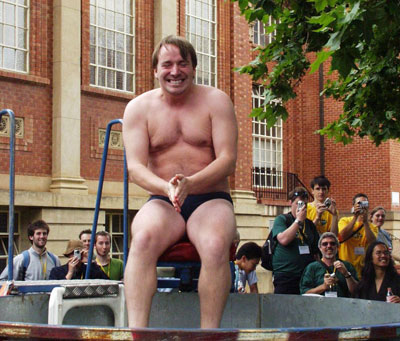
\includegraphics[width=3cm]{images/linustorvaldsspeedo.jpg}
	\end{center}

	Linus Torvalds disse:
	\begin{itemize}
		\item "I don't like debuggers. Never have, probably never will"
		\item "I happen to believe that not having a kernel debugger forces people to
think about their problem on a different level than with a debugger."
		\item "Without a debugger, you tend to think about problems another way."
	\end{itemize}
\end{frame}

\subsection{Como solucionar um problema no kernel}
\begin{frame}
       \frametitle{Como solucionar um problema no kernel}

       \begin{itemize}
               \item Lendo o código
               \item O rei dos depuradores {\tt
printk()}\footnote{muitos mili segundos} ou {\tt
trace\_printk()}\footnote{décimos de microsegundos}
               \item Ftrace, LLTng e Systemtap
               \item {\bf xmon} para PowerPC
       \end{itemize}
       \alert{ E se: }
       \begin{itemize}
               \item O problema for no boot
               \item Se você não sabe onde o problema está ?
               \item Interativo/Step-by-step
               \item Comandos on-demand
       \end{itemize}
\end{frame}

\begin{frame}[containsverbatim]
\footnotesize
\begin{verbatim}
0:mon> e
cpu 0x0: Vector: 700 (Program Check) at [c0000000035af8b0]
   pc: c000000000496dd0: .skb_pull+0x30/0x50
   lr: c0000000004c55ac: .eth_type_trans+0x3c/0x160
 current = 0xc000000039325570
 paca    = 0xc000000000f62500
   pid   = 15772, comm = ftp
kernel BUG at include/linux/skbuff.h:1132!
0:mon> t
[link register   ] c000004c55ac .eth_type_trans+0x3c/0x160
[c00035afb30] c00000e3c6b0 check_legacy_serial_console+0x0/0x10
[c00035afbc0] d000014049e8 .ixgbe_clean_rx_irq+0x578/0x940 [ixgbe]
[c00035afcf0] d00001405dd4 .ixgbe_clean_rxtx_many+0x124/0x280 [ixgbe]
[c00035afdc0] c000004a7788 .net_rx_action+0x168/0x2e0
...
[c00000003e4a7e30] c00000000000852c syscall_exit+0x0/0x40
--- Exception: c01 (System Call) at 0000008078afbb64
\end{verbatim}
\end{frame}

\section{Histórico}
\subsection{Depurando step-by-step}
\begin{frame}
	\frametitle{Depurando step-by-step}
	\begin{itemize}
		\item Surge uma implementação na LinSysSoft no kernel 2.4
		\item Em 2006 a Wind River assume o código e cria o KGDB light
		\item Isto é, depuração estritamente via console serial ({\tt kgdboc})
		\item Depuração via Ethernet é temporariamente cancelada ({\tt kgdboe})
		\item Ingo Molnar adere ao projeto e o KGDB light é aceito \textit{upstream} no kernel 2.6.26 (2008)
	\end{itemize}
\end{frame}

\begin{frame}[containsverbatim]
\small
\begin{center}
\begin{verbatim}
 "This is a slimmed-down and cleaned up version of KGDB that
i've created out of the original patches that we submitted
two weeks ago. I went over the kgdb patches with Thomas and
we cut out everything that we did not like, and cleaned up
the result. KGDB is still just as functional as it was before
(i tested it on 32-bit and 64-bit x86) - and any desired
extra capability or complexity should be added as a delta
improvement, not in this initial merge." --Ingo Molnar

\end{verbatim}
\end{center}
\end{frame}

\subsection{O que é o KGDB}
\begin{frame}
	\frametitle{O que é o KGDB}
	\begin{itemize}
		\item Extensão que provê mecanismo para depurar o kernel usando GDB
		\item São necessárias 2 máquinas (uma estará parada no \textit{breakpoint})
		\item Atualmente, utiliza a porta serial para comunição
		\item Multi-arquitetura (x86, x86-64, ARM, Blackfin, MIPS, SH, PowerPC e SPARC)
		\item Pode ser utilizada em máquinas virtuais
	\end{itemize}
\end{frame}

\section{Funcionamento}
\subsection{Configurações}
\begin{frame}[fragile]
	\frametitle{Configurações}
	\begin{center}
	\begin{itemize}
		\item Habilitar suporte ao KGDB no kernel
		\item Habilitar compilação com \textit{debug info} para informações sobre código fonte
		\item Desabilitar \textit{write protect} kernel para possibilitar inserção de \textit{breakpoints}
	\end{itemize}
	\begin{block}{{\tt \$ make menuconfig}}
	\tiny
	\begin{verbatim}
General setup  --->
    [*] Prompt for development and/or incomplete code/drivers
Kernel hacking  --->
    -*- Magic SysRq key
    [*] Compile the kernel with debug info
    [*] KGDB: kernel debugger  --->
        --- KGDB: kernel debugger
        <*>   KGDB: use kgdb over the serial console
        [ ]   KGDB: internal test suite
        [ ]   KGDB: Allow debugging with traps in notifiers
        [*]   KGDB_KDB: include kdb frontend for kgdb
        [*]     KGDB_KDB: keyboard as input device
    [ ] Write protect kernel read-only data structures
	\end{verbatim}
	\normalsize
	\end{block}
	\end{center}
\end{frame}

\subsection{Parâmetros}
\begin{frame}
       \frametitle{Parâmetros}
        \begin{center}
	\begin{itemize}
		\item \textbf{kgdboc=kbd,kms,\parametro{serial},\parametro{baudrate}}
		\begin{itemize}
			\item \textbf{kbd}: (e não kdb) suporte ao Kernel Debugger
			\item \textbf{kms}: integração ao Kernel Mode Setting, para acessar o console toda vez que entrar em modo depuração
			\item \textbf{\parametro{serial},\parametro{baudrate}}: configuração da interface serial
			\item Parâmetros também configuraveis através de \tt{/sys/module/kgdboc/parameters/kgdboc}
		\end{itemize}
		\item \textbf{kgdbwait}
		\begin{itemize}
			\item Kernel é bloqueado na inicialização aguardando conexão do GDB
			\item Suporte ao KGDB deve estar compilado \textit{built-in}
		\end{itemize}
		\item \textbf{kgdbcon}
		\begin{itemize}
			\item Mensagens do kernel são replicadas no GDB enquanto este estiver conectado
		\end{itemize}
	\end{itemize}
        \end{center}
\end{frame}

\subsection{Demonstração}
\begin{frame}
       \frametitle{Setup}
        \begin{center}
	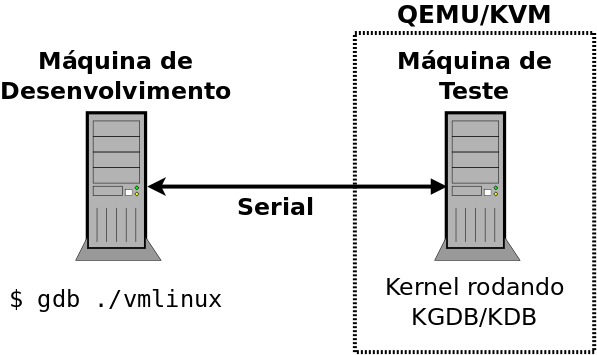
\includegraphics[width=8cm]{images/setup.png}
        \end{center}
\end{frame}

\begin{frame}[fragile]
       \frametitle{Exemplo usando KGDB - \textit{Breakpoints}}
        \begin{center}
	\begin{itemize}
		\item Habilitar KGDB via ttyS0 na máquina de testes
		\tiny
		\begin{verbatim}
# echo ttyS0 > /sys/module/kgdboc/parameters/kgdboc
# echo g > /proc/sysrq-trigger
		\end{verbatim}
		\normalsize
		\item Na máquina de desenvolvimento, conectar GDB (verificar SERIAL utilizada pelo KVM/QEMU) e incluir um breakpoint na função {\tt icmp\_reply}
		\tiny
		\begin{verbatim}
$ gdb ./vmlinux
(gdb) target remote /dev/pts/<SERIAL>
(gdb) break icmp_reply
(gdb) cont
		\end{verbatim}
		\normalsize
		\item Envie um \textit{ping} para a máquina de testes a partir da máquina de desenvolvimento
		\tiny
		\begin{verbatim}
$ ping 192.168.122.218 -c 1
		\end{verbatim}
		\normalsize
	\end{itemize}
        \end{center}
\end{frame}

\begin{frame}[fragile]
       \frametitle{Exemplo usando KGDB - Depurando módulos}
        \begin{center}
	\begin{itemize}
		\item Na máquina de testes, carregar o módulo de rede \textit{dummy}
		\tiny
		\begin{verbatim}
# modprobe dummy
# ifconfig dummy0
# cat /sys/module/dummy/sections/.text
# cat /sys/module/dummy/sections/.data
# echo g > /proc/sysrq-trigger
		\end{verbatim}
		\normalsize
		\item Na máquina de desenvolvimento, adicionar ao GDB os endereços das seções ELF do módulo carregado e um \textit{breakpoint} para a função {\tt dummy\_set\_address}
		\tiny
		\begin{verbatim}
$ gdb ./vmlinux
(gdb) target remote /dev/pts/<SERIAL>
(gdb) add-symbol-file drivers/net/dummy.o <ENDEREÇO .text> -s .data <ENDEREÇO .data>
(gdb) break dummy_set_address
(gdb) cont
		\end{verbatim}
		\normalsize
		\item Na máquina de testes, configurar o endereço MAC da interface {\tt dummy0}
		\tiny
		\begin{verbatim}
# ifconfig dummy0 hw ether 00:00:00:00:00:01
		\end{verbatim}
		\normalsize
		\item Na máquina de desenvolvimento, redefinir o MTU na estrutura {\tt dev}
		\tiny
		\begin{verbatim}
(gdb) set dev->mtu = 1499
(gdb) cont
		\end{verbatim}
		\normalsize
	\end{itemize}
        \end{center}
\end{frame}

\section{KDB}
\subsection{O que é o KDB}
\begin{frame}
       \frametitle{O que é o KDB}
        \begin{center}
        \begin{itemize}
	    \item Kernel DeBugger é um depurador \textit{built-in} mantido pela SGI como \textit{patch} externo desde Linux 2.2
	    \item Não necessita de uma segunda máquina para depuração
	    \item Utiliza apenas teclado + console texto VGA
	    \item Não é um depurador em nível de código
	    \item Útil para verificar {\tt dmesg}, {\tt lsmod}, {\tt ps}, \textit{stack trace}, estado dos registradores
	    \item Também possui suporte a \textit{breakpoints} e modificações na memória
	    \item Acessível através do KGDB (comando {\tt monitor})
	\end{itemize}
        \end{center}
\end{frame}

\subsection{Demonstração}
\begin{frame}[fragile]
       \frametitle{Exemplo usando KDB - \textit{Breakpoints}}
        \begin{center}
	\begin{itemize}
		\item A partir do console da máquina de testes, execute
		\tiny
		\begin{verbatim}
# echo kbd,ttyS0 > /sys/module/kgdboc/parameters/kgdboc
# echo g > /proc/sysrq-trigger
		\end{verbatim}
		\normalsize
		\item O sistema é direcionado para o prompt do KDB. Então inserimos um \textit{breakpoint} na \textit{syscall} {\tt sys\_mkdir}
		\tiny
		\begin{verbatim}
[0]kdb> bp sys_mkdir
[0]kdb> go
		\end{verbatim}
		\normalsize
		\item De volta ao prompt do sistema, execute um comando mkdir
		\tiny
		\begin{verbatim}
# mkdir dirteste
		\end{verbatim}
		\normalsize
	\end{itemize}
        \end{center}
\end{frame}

\begin{frame}
       \frametitle{Outros Exemplos}
        \begin{center}
	\begin{itemize}
	\item \textit{Breakpoint} em outras \textit{syscalls} como {\tt sys\_sync} (utilizada pelo {\tt sync})
	\item Utilizando {\tt monitor} do KGDB para matar processos via KDB
	\item Carregar um módulo exemplo com algum \textit{bug} providencial
	\end{itemize}
        \end{center}
\end{frame}

\section{Futuro}
\begin{frame}
       \frametitle{Futuro}
        \begin{center}
        \begin{itemize}
		\item Conclusão do \textit{merge} KGDB + KDB (2.6.35)
		\item Integração com KMS (Kernel Mode Setting)
		\item kgdbou (KGDB over USB)
		\begin{itemize}
		    \item Estabilizar suporte USB Console
		\end{itemize}
		\item kgdboe v2 (KGDB over Ethernet)
		\begin{itemize}
		    \item Melhorias nos drivers de rede (problemas com preempção + \textit{locks})
		    \item Ou hardware com fila dedicada (ex.: e1000e)
		\end{itemize}
	\end{itemize}
        \end{center}
\end{frame}

\section{Referências}
\begin{frame}
       \frametitle{Referências}
        \begin{center}
        \begin{itemize}
		\item \textbf{KGDB Wiki} \\
		http://kgdb.wiki.kernel.org

		\item \textbf{Using kgdb, kdb and the kernel debugger internals} \\
		http://kernel.org/pub/linux/kernel/people/jwessel/kdb/

		\item \textbf{IBM developerWorks - Mastering Linux debugging techniques} \\
		http://www.ibm.com/developerworks/linux/library/l-debug/

		\item \textbf{KGDB Mailing List} \\
		https://lists.sourceforge.net/lists/listinfo/kgdb-bugreport
	\end{itemize}
        \end{center}
\end{frame}

\section{}
\begin{frame}
	\begin{center}
	\LARGE
	\alert{Obrigado!}

	Dúvidas?


	\vspace{2\baselineskip}

	\small
	Edjunior Machado \\ {\tt edjunior@gmail.com / emachado@linux.vnet.ibm.com} \\
	Breno Leitão \\ {\tt breno.leitao@gmail.com / leitao@linux.vnet.ibm.com}
	\end{center}
\end{frame}

\end{document}

